\documentclass{lab_class}

\usepackage{fancyhdr}
\pagestyle{fancy}
\rhead{П.\,Ю. Смирнов, 687 гр.}
\lhead{Лабораторная работа № 3.2.5, МФТИ, осень 2017}

\begin{document}

{\Large 3.2.5 --  Вынужденные колебания в электрическом контуре.}

\paragraph{Цель работы.}
Исследование вынужденных колебаний и процессов их установления.
В работе используются: генератор звуковой частоты, осциллограф, вольтметр, частотометр, ёмкость, индуктивность, магазин сопротивлений, универсальный мост.

\paragraph{Теоретическая часть.}
В данной работе будем рассматривать колебания в электрическом колебательном контуре под воздействием внешней ЭДС, гармонически изменяющейся во времени.
 
\begin{wrapfigure}[12]{r}{6cm}
\centering
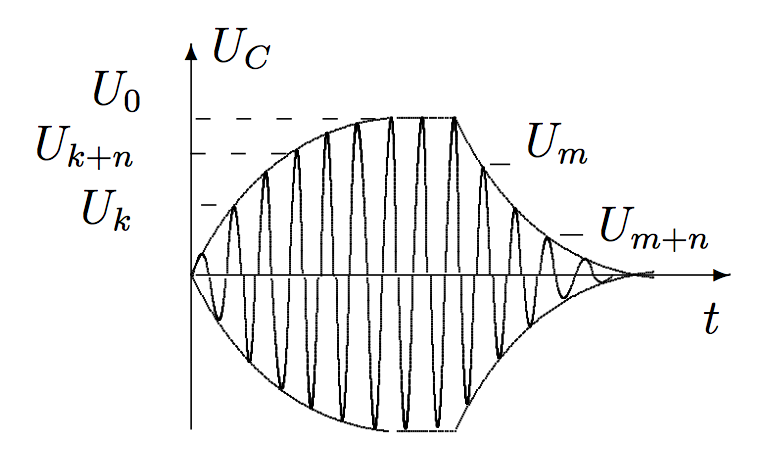
\includegraphics[width=6cm]{Fig3.png}
\caption{Нарастание и затухание вынужденных колебаний}
\end{wrapfigure}

Получаем, что при подключении внешнего источника возникнут колебания, которые будем рассматривать как решение дифференциального уравнения:
\begin{equation}
L\ddot{I} + R \dot{I} + \dfrac{I}{C} = - \ef \Omega \sin \Omega t,
\end{equation}
в качестве суперпозиции двух синусоид: 
\begin{equation}
I = Be^{-\gamma t} \sin (wt-\theta) + \dfrac{\ef \Omega}{L \rho_0} \sin (\Omega t - \psi),
\end{equation}
одна из которых с частотой собственных колебаний контура $\omega$ и амплитудой, экспоненциально убывающей со временем; вторая - с частотой внешнего источника и постоянной амплитудой. Однако со временем собственные колебания затухают, и в контуре устанавливаются вынужденные колебания. А их амплитуда максимальна, когда знаменатель второй синусоиды $\rho_0 = \sqrt{(\omega_0^2 - \Omega^2_0)^2 + (2\gamma \Omega)^2}$ минимален, то есть $\omega_0 = \Omega$ (частота внешнего сигнала совпадает с собственной частотой контура). Это явление и называется \textit{резонансом}. Зависимость амплитуды колебаний от частоты внешнего напряжения называется \textit{резонансной кривой}.

\paragraph{Резонансная кривая колебательного контура.}
\begin{wrapfigure}[10]{l}{6cm}
\centering
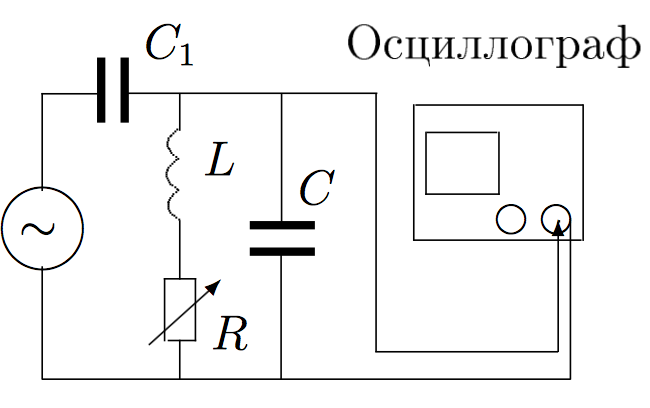
\includegraphics[width=5cm]{Fig2.png}
\caption{Схема установки}
\end{wrapfigure} 

Мы можем снять зависимость амплитуды напряжения на резисторе $R$ от частоты на генераторе (при постоянной амплитуде выходного напряжения), однако для этого выходное сопротивление генератора должно быть много меньше импеданса контура. Для этого в цепи используется конденсатор $C_1$. И в таком случае импеданс внешней по отношению к контуру цепи был гораздо больше импеданса самого контура вблизи резонанса:

$$\dfrac{1}{\omega C_1} \gg |Z_\text{рез}| = \dfrac{L}{RC} $$

\paragraph{Процессы установления и затухания колебаний.}
Добротность контура можно определить и другими способами, например, по скорости затухания свободных колебаний. Подавая на контур цуги синусоид конечной длины, можно наблюдать процессы установления и затухания колебаний в контуре. И те, и другие могут быть использованы для определения добротности контура по скорости нарастания/затухания напряжения:

$$\Theta = \dfrac{1}{n} \ln \dfrac{U_0 - U_k}{U_0-U_{k+n}} $$

Измеряя амплитуды напряжения в какой-нибудь момент времени и через n периодов, можем посчитать добротность по формуле:
$$Q = \dfrac{\pi}{\gamma 	T} = \dfrac{\pi}{\Theta}$$

\paragraph{Установка и параметры измерения.}
\begin{figure}[H]
\centering
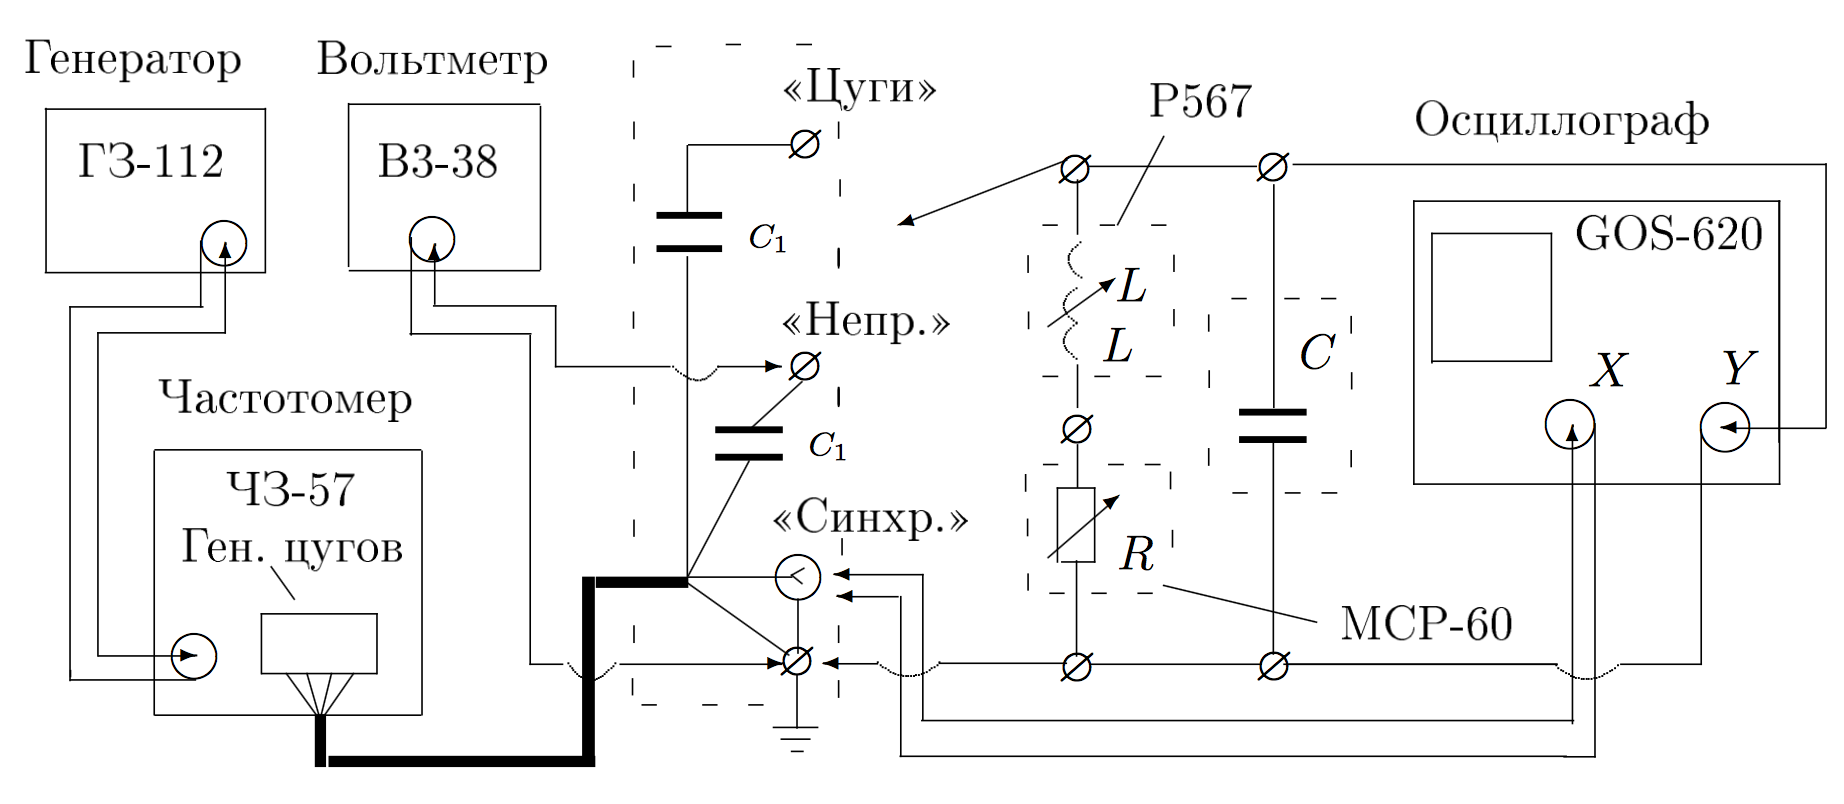
\includegraphics[width = 0.9 \textwidth]{Fig.png}
\caption{Схема экспериментальной установки для исследования вынужденных колебаний}
\end{figure}

Идеальная схема, изображённая на рисунке 2, не соответствует действительности.  Элементы цепи не идеальны и имеют паразитные сопротивления. Измерим все величины с помощью RLC – моста:

$$R_L = 29.3 \; \Ohm\footnote{Заметим, что $R_L$ зависит от частоты. В диапазоне 50 -- 1500 \hz \; абсолютное изменение порядка ома.}, \; L = 99.9 \; \sm \H, \; C = 100.0 \; \sn \F, \; R = 100.0 \; \Ohm$$

Снимем зависимость напряжения на конденсаторе от входной частоты, и получим таким образом резонансную кривую. Рассчитаем добротность контура при разных значениях резистора по известной формуле:

$$Q = \dfrac{\nu_0}{\Delta \nu}$$

\begin{table}[H]
\centering
\resizebox{\textwidth}{!}{
\begin{tabular}{|c|c|c|c|c|c|c|c|c|c|c|c|c|c|c|c|c|}
\hline
U, \V  & 0.83  & 0.64  & 0.45  & 0.33  & 0.25  & 0.20  & 0.28  & 0.48  & 0.91  & 0.80  & 0.70  & 0.60  & 0.50  & 0.40  & 0.30  & 0.20  \\ \hline
$\nu$, \hz & 1594  & 1600  & 1631  & 1657  & 1692  & 1727  & 1673  & 1626  & 1561  & 1553  & 1546  & 1538  & 1528  & 1515  & 1493  & 1455  \\ \hline
$\nu/ \nu_0$  & 1.02  & 1.02  & 1.04  & 1.06  & 1.08  & 1.10  & 1.07  & 1.04  & 1.00  & 0.99  & 0.99  & 0.98  & 0.97  & 0.97  & 0.95  & 0.93  \\ \hline
$U/U_0$  & 0.91  & 0.70  & 0.49  & 0.36  & 0.27  & 0.22  & 0.30  & 0.52  & 1.0  & 0.88  & 0.77  & 0.66  & 0.55  & 0.44  & 0.33  & 0.22  \\ \hline
\end{tabular}%
}
\caption{Полученные значения при R = 0 \Ohm}
\end{table}

\begin{table}[H]
\centering
\resizebox{\textwidth}{!}{
\begin{tabular}{|c|c|c|c|c|c|c|c|c|c|c|c|c|c|c|c|c|}
\hline
U, \V  & 0.82  & 0.72  & 0.60  & 0.50  & 0.40  & 0.30  & 0.20  & 0.72  & 0.60  & 0.50  & 0.40  & 0.30  & 0.20  \\ \hline
$\nu$, \hz & 1578  & 1523  & 1490  & 1456  & 1418  & 1365  & 1272  & 1644  & 1692  & 1744  & 1817  & 1940  & 2330  \\ \hline
$\nu/ \nu_0$  & 1.00  & 0.96  & 0.94  & 0.92  & 0.89  & 0.86  & 0.80  & 1.04  & 1.07  & 1.10  & 1.15  & 1.23  & 1.47  \\ \hline
$U/U_0$  & 1.0  & 0.87  & 0.73  & 0.61  & 0.48  & 0.36  & 0.24  & 0.87  & 0.73  & 0.61  & 0.48  & 0.36  & 0.24  \\ \hline
\end{tabular}%
}
\caption{Полученные значения при R = 100 \Ohm}
\end{table}

\paragraph*{Экспериментальные значения добротностей:}
\begin{gather*}
Q_{R=0} = 25.1 \pm 1.2 \\
Q_{R=100} = 7.3 \pm 0.4
\end{gather*}

\begin{table}[H]
\centering
\begin{tabular}{|c|c|c|c|c|c|c|}
\hline
                    & \multicolumn{3}{c|}{Возрастание} & \multicolumn{3}{c|}{Затухание} \\ \hline
$R, \; \Ohm$        & \multicolumn{6}{c|}{0} \\ \hline
$U_{n}, \; \sm \V$  & 200    & 400    & 400     & 200    & 640   & 640 \\ \hline
$U_{k+n},\; \sm \V$ & 440    & 640    & 680     & 160    & 440   & 120  \\ \hline
$U_0, \; \sm \V$    & \multicolumn{3}{c|}{740}  & \multicolumn{3}{c|}{-} \\ \hline
k                   & 5      & 10     & 15      & 5       & 10    & 15    \\ \hline
Q                   & 26.7   & 25.6   & 27.1    & 24.2    & 26.7    & 28.1    \\ \hline
\end{tabular}
\caption{Измерение добротности по нарастанию и затуханию при R = 0 \Ohm}
\end{table}

\begin{table}[H]
\centering
\begin{tabular}{|c|c|c|c|c|c|c|}
\hline
                    & \multicolumn{3}{c|}{Возрастание} & \multicolumn{3}{c|}{Затухание} \\ \hline
$R, \; \Ohm$        & \multicolumn{6}{c|}{100} \\ \hline
$U_{n}, \; \sm \V$  & 40    & 100    & 100     & 200    & 200   & 110 \\ \hline
$U_{k+n},\; \sm \V$ & 180    & 190    & 170     & 80    & 20   & 30  \\ \hline
$U_0, \; \sm \V$    & \multicolumn{3}{c|}{200}  & \multicolumn{3}{c|}{-} \\ \hline
k                   & 5      & 10     & 3      & 3       & 6    & 3    \\ \hline
Q                   & 7.5   & 8.6   & 7.8    & 10.3      & 8.2    & 7.2    \\ \hline
\end{tabular}
\caption{Измерение добротности по нарастанию и затуханию при R = 100 \Ohm}
\end{table}

\paragraph*{Экспериментальные значения добротности (нарастание напряжения):}
\begin{gather*}
Q_{R=0} = 26.4 \pm 0.7 \\
Q_{R=100} = 7.9 \pm 0.5
\end{gather*}

\paragraph*{Экспериментальные значения добротности (убывание напряжения):}
\begin{gather*}
Q_{R=0} = 26.3 \pm 1.1 \\
Q_{R=100} = 8.5 \pm 1.8
\end{gather*}

%\paragraph*{Сравнение экспериментальных значений добротности, полученных разными методами}
\begin{table}[H]
\centering
\begin{tabular}{|c|c|c|c|}
\hline
            & Резонансная кривая & Нарастание     & Убывание     \\ \hline
$Q_{R=0}$   & $25.1 \pm 1.2$     & $26.4 \pm 0.7$ & $26.3 \pm 1.1$ \\ \hline
$Q_{R=100}$ & $7.3 \pm 0.4$      & $7.9 \pm 0.5$  & $8.5 \pm 1.8$  \\ \hline
\end{tabular}
\caption{Сравнение экспериментальных значений добротности, полученных разными методами}
\end{table}

\paragraph{Вывод.}
Были изучены законы, описывающие переходные процессы в резонансном контуре, изучена резонансная кривая и определение добротности из разных физических соображений.

\bigskip

\begin{figure}[H]
\centering
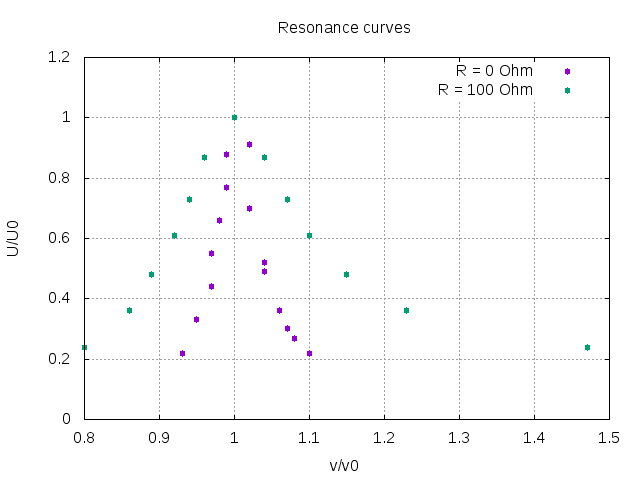
\includegraphics[width = 0.9 \textwidth]{graph.png}
\caption{Резонансные кривые для $R = 100 \; \Ohm$ и $R = 0 \; \Ohm$}
\end{figure}

\end{document}